\documentclass[letterpaper]{article}
\usepackage{amsmath}
\usepackage{amsfonts}
\usepackage{fontspec}
\usepackage{graphicx}
\usepackage{float}		%\begin{figure}[H] <- agrega el H
\usepackage{multirow}
\usepackage{multicol}
\usepackage{indentfirst}
\usepackage{caption} %comando \ContinuedFloat
\usepackage{array} %paquete para tabular
\usepackage{subcaption} %subfiguras y continuación de figura
\usepackage{pstricks-add}
\usepackage{bm}
\usepackage{enumitem} %cara utilizar distintos enumerate item


\newcolumntype{P}[1]{>{\centering\arraybackslash}p{#1}} % P{} (mayúscula) en vez de p{} (minúscula)
\newcommand{\vect}[1]{\boldsymbol{#1}} %notación vector \vect{•}
\renewcommand{\contentsname}{Índice}
\renewcommand{\figurename}{Figura}
\renewcommand{\tablename}{Tabla}
\renewcommand\refname{Referencias}

%%% quita los ":" del \caption
\makeatletter
\long\def\@makecaption#1#2{%
\vskip\abovecaptionskip
\sbox\@tempboxa{#1. #2}%
\ifdim \wd\@tempboxa >\hsize
#1. #2\par
\else
\global \@minipagefalse
\hb@xt@\hsize{\hfil\box\@tempboxa\hfil}%
\fi
\vskip\belowcaptionskip}
\makeatother
%%%%%%%%%%%%%%%%%%%%%%%%%


\pagestyle{plain}


%FORMATO PÁGINA
%\hoffset
\voffset=-2cm
\oddsidemargin=0.8cm
%\evensidemargin
%\topmargin 		%entre sup y encab
%\headheight		%tamaño encabezado
%\headsep			%sep encab y text
\textheight=23cm		%altura texto
\textwidth=15cm		%ancho texto
%\marginparsep	%sep notmargen y text
%\marginparwidth	%ancho nota al marg
\footskip=1cm		%pie de pag

\begin{document}

\thispagestyle{empty}

\hspace{-5mm}
\begin{minipage}[c]{7cm}
\centering

\includegraphics[width=4cm]{logoutfsm.jpg} \\
Universidad Técnica Federico Santa María
\end{minipage}
\hfill
\hspace{20mm}
\begin{minipage}[c]{7cm}
\centering

\includegraphics[width=4cm]{logomec1.jpg} \\
Departamento de Ingenieria Mecánica
\end{minipage}

\begin{center}
\vfill
 \Huge{{\bf Proyecto 1 }} \\ \vspace{1cm} 
 \Huge{Dinámica de fluidos computacional}
\vfill
\end{center}

\vfill \hfill
\begin{tabular}{l @{ : } l}
Nombre &   Ignacio Apablaza \\
Rol & 201141007-6  \\
Profesores & Romain Gers \\
			& Olivier Skurtys \\
Asignatura & IPM468 \\
\end{tabular}

\newpage
%---------------------------------------------


\tableofcontents


\newpage
%---------------------------------------------

\section{Resumen}






\newpage
%---------------------------------------------

\section{Introducción}







\newpage
%---------------------------------------------

\section{Metodología}
Ecuación de onda

\begin{equation}
\dfrac{\partial^2 y}{\partial t^2} - \gamma \dfrac{\partial^2 y}{\partial x^2} = f
\end{equation} 

Esquema de discretización Newmark

\begin{equation}
v = \dfrac{\partial u}{\partial t}
\end{equation}

Luego, el desarrollo de Taylor de $v(t+ \Delta t) = t^{n+1}$ para un paso de tiempo $\Delta t$ es

\begin{equation}
v^{n+1} = v^{n} + \Delta t \dfrac{\partial v}{\partial t} (t= \xi)
\end{equation}

para $\xi \in [t,t+\Delta t]$ .como

\begin{equation}
\dfrac{\partial v}{partial t} = \dfrac{\partial^2 u}{\partial t^2} = \gamma \dfrac{\partial^2 u}{\partial x^2} + f 
\end{equation}

Reemplazando en la (ECUACION!) se tiene 

\newpage
%---------------------------------------------

\section{Desarrollo y Análisis} \label{DESARROLLO_Y_ANALISIS}

%----

\subsection{Ejercicios en Fortran}
\subsubsection{Ejercicio 1}

Sea $A(n)$ un número real tal que
\begin{equation}
A(n) = \sum_{n=1}^\infty \dfrac{1}{n}
\end{equation}
Se implementa una programa en Fortran que permite calcular y graficar $A(n)$ para ciertos valores de $n$. En la Figura \ref{fig_P1_1_1} se grafica $A$ para simple y doble precisión. En la Figura \ref{fig_P1_1_2} Para doble y cuadruple precisión

\begin{figure} [H]
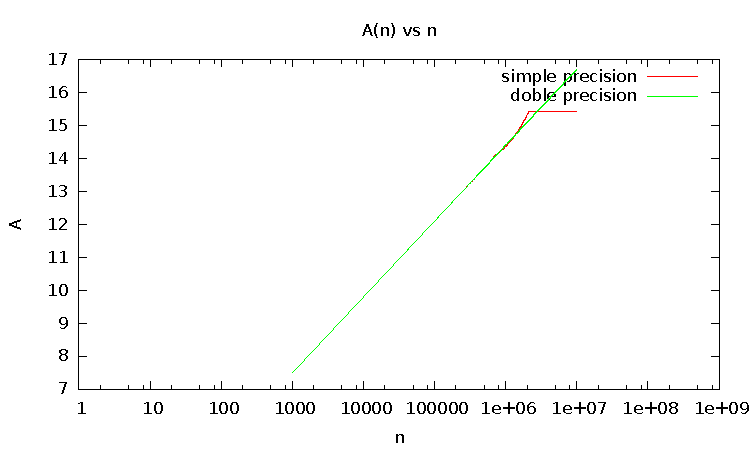
\includegraphics{./parte2/graficos/grafico_p1_1.pdf}
\caption{} \label{fig_P1_1_1}
\end{figure}

\begin{figure} [H]
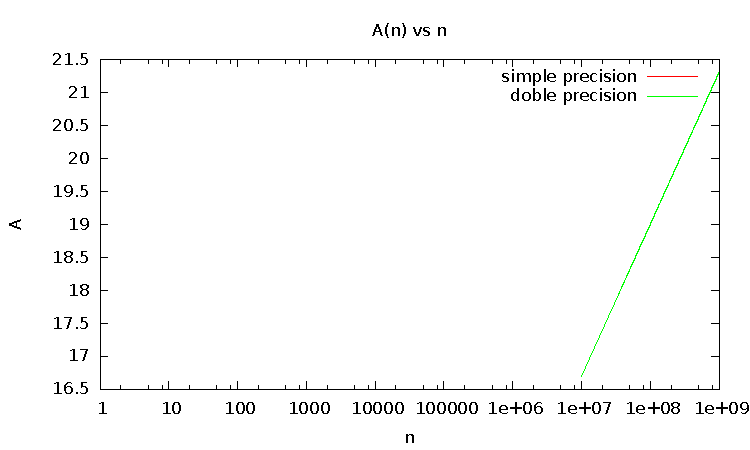
\includegraphics{./parte2/graficos/grafico_p1_2.pdf}
\caption{} \label{fig_P1_1_2}
\end{figure}

%----------------------------------------------
\subsubsection{Ejercicio 2}
Se implementa una rutina en Fortran que permite calcular los $n+1$ valores de la serie Fibonacci
\begin{equation}
u_{n+1} = u_{n} + u_{n-1} \hspace{1cm} \mbox{tal que} \hspace{0,5cm} u_0=0 \hspace{0,1cm} ; \hspace{0,1cm} u_1=1
\end{equation}
La serie se grafica para $n=100$

\begin{figure} [H]
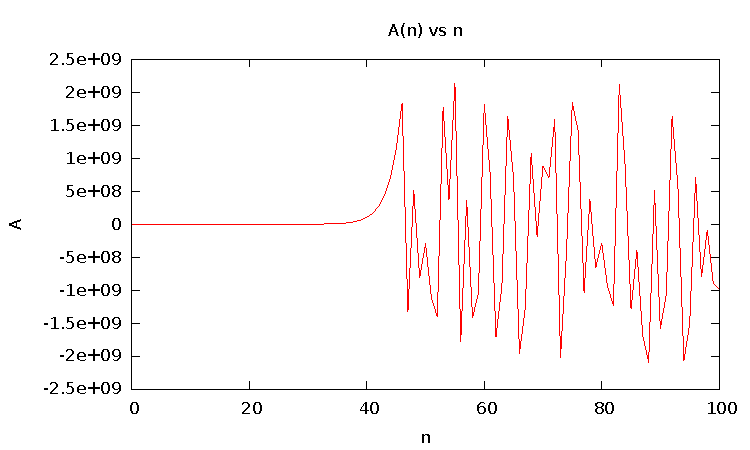
\includegraphics{./parte2/graficos/grafico_p2.pdf}
\caption{} \label{fig_P1_2}
\end{figure}

%----

\subsection{Estudio del comportamiento mecánico de una arteria}
%Estudio del comportamiento mecánico de una arteria

\subsection{Parte 1: Movimiento de una pared arterial}

Una arteria puede modelarse por un cilindro flexible de base circular, longitud $L$, radio $R_0$, cuyas paredes poseen un espesor $H$. Se supone que está constituido de un material elástico, incompresible, homogéneo e isotrópico. \\

Un modelo simplificado que describe el comportamiento mecánico de la pared arterial en interacción con el flujo sanguíneo se obtiene considerando que el cilindro es constituido por un conjunto de anillos independientes uno de otros. De esta manera se puede despreciar las interacciones longitudinales y axiales a lo largo de la arteria. Luego, se supone que la arteria se deforma solamente en la dirección radial. \\

El radio de la arteria está dado por,
\begin{equation}
R(t) = R_0 + y(t)
\end{equation}
donde $y(t)$ es la deformación radial en función del tiempo $t$. Al aplicar la ley de Newton en el sistema de anillo independientes conduce a una ecuación que permite modelar el comportamiento mecánico de la pared de la arteria en función del tiempo,
\begin{equation} \label{PROBLEMA_PARTE2}
\dfrac{d^2 y(t)}{dt^2} + \beta \dfrac{dy(t)}{dt} + \alpha y(t) = \gamma (p(t)-p_0)
\end{equation}
donde,
\begin{equation}
\alpha = \dfrac{E}{\rho_w R^2_0} \hspace{0,5cm} \gamma = \dfrac{1}{\rho_w H} \hspace{0,5cm} \beta = \mbox{constante} > 0 
\end{equation}

Particularmente se modela la variación de la presión a lo largo de la arteria como una función sinusoidal que depende de la posición $x$ y el instante de tiempo $t$,
\begin{equation} \label{FUENTE_PARTE2}
(p-p_0) = x \Delta p  \left( a + b cos( \omega_0 t ) \right)
\end{equation} 

Se calcula numericamente la ecuación (\ref{PROBLEMA_PARTE2}) con el término fuente (\ref{FUENTE_PARTE2}).  Se uyilizan los siguientes valores realistas para los parámetros físicos:
\begin{table} [H]
\centering
\begin{tabular}{llll}
$L$		& = $5 \times 10 ^ {-2}$ m 				&	$b$	 		&= $133.32$ N m $^{-2}$ \\
$R_0$	& = $5 \times 10 ^ {-3}$ m 				&	$a$		 	&= $1333.2$ N m $^{-2}$ \\
$\rho_w$& = $1 \times 10 ^ {3}$ kg m $^{-3}$ 	&	$\Delta p$ 	&= $33.33$ N m $^{-2}$ \\
$H$		& = $3 \times 10 ^ {-4}$ m 				&	$w_0$ 		&= $2 \pi / 0.8$ \\
$E$		& = $9 \times 10 ^ {5}$ N m $^{-2}$ 	&				&
\end{tabular}
\caption{Parametros utilizados para la simulación 1} \label{PARAMETROS_PARTE2}
\end{table}
Y considerando a su vez dos parametros de $\beta$:
\begin{enumerate}[label=(\alph*)]
\item $\beta = \sqrt{ \alpha }$ 
\item $\beta = \alpha$
\end{enumerate}
Se reescribe la ecuación (\ref{PROBLEMA_PARTE2}) como un sustema de ecuaciones lineales. En forma matricial,
\begin{equation} \label{•}\vect{A} \vec{y} + \vec{b}
\end{equation}
donde $\vec{y} = \begin{vmatrix} y & y' \end{vmatrix}^T$ ($T$ significa transpuesta), y $\vec{b}(t)$ es un vector fuente dependiente del tiempo $t$. La matriz $\vect{A}$ resultante es,
\begin{equation}
\vect{A} = \begin{pmatrix}
0 & 1 \\ -\alpha & -\beta
\end{pmatrix}
\end{equation}
Los valores propios de $\vect{A}$ se obtienen del desarrollo del polinomio característico,
\begin{equation}
det(\vect{A} - \Omega \vect{I}) = \begin{vmatrix}
-\Omega & 1 \\
-\alpha & -\Omega -\beta 
\end{vmatrix} \rightarrow \alpha \Omega^2 + \beta \Omega + 1 = 0
\end{equation}
Luego, los valores propios se calculan como la raíz del polinomio,
\begin{equation}
\Omega_{1,2} = \dfrac{( -\beta \pm \sqrt{ \beta^2 - 4 \alpha})}{2}
\end{equation}

Notar que para valores de $\beta \geq 2\sqrt{\alpha}$ ambos valores, $\Omega_1$ y $\Omega_2$, resultan reales y negativos, mientras que para valores de $\beta < 2\sqrt{\alpha}$ ambos autovalores resultan números complejos con su componente real negativa. \\

Se implementa una subrutina que permite calcular los valores propios de la matriz $\vect{A}$. Utilizando los valores de la Tabla \ref{PARAMETROS_PARTE2} se obtiene:
\begin{enumerate} [label=(\alph*)]
\item $\beta = \sqrt{\alpha} = 6.0 \times 10^3 $
\begin{equation}
\vect{A} = \begin{pmatrix} 0 & 1 \\ 36.0 \times 10^6 & 6.0 \times 10^3 \end{pmatrix} \rightarrow 
\begin{matrix} \Omega_1 = & -3000.00 + 5196.15 i \\ \Omega_2 = & -3000.00 - 5196.15 i \end{matrix}
\end{equation} 
\item $\beta = \alpha =  36.0 \times 10^6 $
\begin{equation}
\vect{A} = \begin{pmatrix} 0 & 1 \\ 36.0 \times 10^6 & 36.0 \times 10^6 \end{pmatrix} \rightarrow 
\begin{matrix} \Omega_1 = & -1.0 \\ \Omega_2 = & -36.0 \times 10^6 \end{matrix}
\end{equation} 
\end{enumerate}

%------------------------------------

\subsubsection{Euler Implicito} 

\paragraph{Discretización de la ecuación diferencial}
Se implementa una subrutina que permite calcular la ecuacion (\ref{PROBLEMA_PARTE2}) usando el método de Euler Implícito para dos valores de $\beta$. Sea $y(x,t) = y^n_j$ y $\partial y / \partial t (x,t) = z^n_j$, recurriendo a la expresión (\ref{PROBLEMA_PARTE2_CORREGIDO}) e implementando un esquema de integración implícito se tiene que,
\begin{align}
\dfrac{y^n - y^{n-1}}{\Delta t} &= z^n \\
\dfrac{z^n - z^{n-1}}{\Delta t} &= -\alpha y^n - \beta z^n + \gamma (p_n-p_0)
\end{align}

Reordenando los valores en los pasos de tiempo $n$ y $n-1$ en los lados izquierdo y derecho respectivamente, se expresa la relación anterior en forma matricial como,
\begin{equation}
\vect{A} \cdot \begin{Bmatrix}
y^n \\ z^n
\end{Bmatrix} =
\begin{Bmatrix}
y^{n-1} \\ z^{n-1}
\end{Bmatrix} +
\Delta t \begin{Bmatrix}
0 \\ \gamma (p_n-p_0)
\end{Bmatrix}
\end{equation}
donde,
\begin{equation}
\vect{A} = \begin{pmatrix}
1 & -\Delta t \\
\Delta t \alpha & 1+ \Delta t \beta
\end{pmatrix}
\end{equation}

Despenjando las incognitas $\begin{Bmatrix} y^n & z^n \end{Bmatrix} ^T$ se obtiene,
\begin{equation}
\begin{Bmatrix}
y^n \\ z^n
\end{Bmatrix} =
\vect{A}^{-1} \cdot \begin{Bmatrix}
y^{n-1} \\ z^{n-1}
\end{Bmatrix} +
\Delta t \vect{A}^{-1} \cdot  \begin{Bmatrix}
0 \\ \gamma (p_n-p_0)
\end{Bmatrix}
\end{equation}
donde
\begin{equation}
\vect{A}^{-1} = 
\dfrac{1}{1 + \beta \Delta t + \alpha (\Delta t) ^ 2}
\begin{pmatrix}
1+\beta \Delta t & \Delta t \\
-\Delta t \alpha & 1 
\end{pmatrix}
\end{equation}

\paragraph{Estabilidad de la solución}
Se quiere estudiar la estabilidad de la solución transiente de (\ref{PROBLEMA_PARTE2_CORREGIDO}). Para ello se recurre a las expresiones (\ref{analisis_espectral_general}) y (\ref{analisis_espectral_descompuesto}). Luego,
\begin{equation}
\dfrac{d \vec{U}}{d t} = \vect{S} \vec{U} + \vec{Q} \rightarrow \left\{ \begin{matrix}
( y^{n+1} - y^n ) /  \Delta t  = \Omega_1 y^{n+1} \\
( z^{n+1} - z^n ) /  \Delta t  = \Omega_2 z^{n+1}
\end{matrix} \right.
\end{equation}
Despejando los terminos evaluados en $t_{n+1}$ en la izquierda de la ecuación
\begin{align}
y^{n+1} &= \dfrac{ 1 }{ 1 - \Delta t \Omega_1 } y^n \\
z^{n+1} &= \dfrac{ 1 }{ 1 - \Delta t \Omega_2 } z^n
\end{align}
Se define $z_{pj}$ como una aproximación de $G(\Omega_j)$ descrito en la Sección \ref{analisis_espectral_seccion}. 
\begin{equation}
\begin{matrix}
G(\Omega_1) \approx z_{py} = \dfrac{ 1 }{ 1 - \Delta t \Omega_1 } \\
G(\Omega_2) \approx z_{pz} = \dfrac{ 1 }{ 1 - \Delta t \Omega_2 }
\end{matrix}
\end{equation}
Es de interés conocer el módulo de $z_p$. La condición de estabilidad se garantiza por el cumplimiento de las restricciones expuestas en las ecuaciones (\ref{convg_1}) y (\ref{convg_2})
\begin{align}
z_p &= \dfrac{1}{1-\Omega_j \Delta t} \notag \\
&= \dfrac{1}{ \left[ 1-\Re(\Omega_j) \Delta t \right] - \left[ \Im(\Omega_j) \Delta t \right] i } \notag \\
&= \dfrac{\left[ 1- \Re(\Omega_j) \Delta t \right] + \left[ \Im(\Omega_j) \Delta t \right] i }{ \left[ 1-\Re(\Omega_j) \Delta t \right]^2 + \left[ \Im(\Omega_j) \Delta t \right]^2}
\end{align}
Entonces,
\begin{equation}
||z_p|| = \dfrac{ \sqrt{ \left[ 1-\Re(\Omega_j) \Delta t \right]^2 + \left[ \Im(\Omega_j) \Delta t \right]^2 } } { \left[ 1- \Re(\Omega_j) \Delta t \right]^2 + \left[ \Im(\Omega_j) \Delta t \right]^2}
\end{equation}
Se observa que $||z_p|| \leq 1 , \hspace{0,2cm} \forall \Omega_j \in \mathbb{C} : \Re(\Omega_j)<0$. Es decir, la solución es incondicionalmente convergente si la parte real de los $j$-ésimos valores propios $\Omega_j$ son menores a cero. A continuación me muestra el cálculo de $\Omega$ para $\beta=\sqrt{\alpha}$ y $\beta=\alpha$ para pasos de tiempo $\Delta t = 10^{-4}$ y $\Delta t = 0.1$. En las Figura \ref{euler_S1_b1} y \ref{euler_S1_b2} se grafica la solución obtenida por la subrutina para $\beta=\sqrt{\alpha}$ y $\beta=\alpha$, respectivamente.  

\subsubsection{Crank Nicolson}

\paragraph{Discretización de la ecuación diferencial} Se utiliza una subrutina que implementa el esquema de Crank Nicolson para la resolución del problema (\ref{PROBLEMA_PARTE2}). Al igual que en el caso anterior se resuelve el problema equivalente (\ref{PROBLEMA_PARTE2_CORREGIDO})

\begin{align}
\dfrac{y^{n+1}-y^n}{\Delta t} & = \dfrac{1}{2} \left( z^{n+1} + z^n \right) \\
\dfrac{z^{n+1}-z^n}{\Delta t} &= \dfrac{1}{2} \left( -\alpha y^{n+1} - \beta y^{n+1} + \gamma (p_{n+1}-p_0) \right) + \dfrac{1}{2} \left( -\alpha y^{n} - \beta y^{n} + \gamma (p_{n}-p_0) \right)  
\end{align}
La relación anterior se escribe en forma matricial,
\begin{equation}
\vect{A} \cdot
\begin{Bmatrix}
y^{n+1} \\ z^{n+1}
\end{Bmatrix} =
\vect{B} \cdot
\begin{Bmatrix}
y^n \\ z^n
\end{Bmatrix} + \dfrac{\Delta t}{2}
\begin{Bmatrix}
0 \\ \left( \gamma (p_{n+1}-p_0) + \gamma (p_{n}-p_0) \right)
\end{Bmatrix}
\end{equation}
donde,
\begin{equation}
\vect{A} = \begin{pmatrix}
1 & -\Delta t /2 \\
\alpha \Delta t / 2 & 1+ \beta \Delta t / 2
\end{pmatrix} 
\end{equation}

\begin{equation}
\vect{B} = \begin{pmatrix}
1 & \Delta t / 2 \\
-\alpha \Delta t / 2 & 1-\beta \Delta t / 2
\end{pmatrix}
\end{equation}
Despejando las variables incognitas $y^{n+1}$ y $z^{n+1}$ se obtiene,
\begin{equation}
\begin{Bmatrix}
y^{n+1} \\ z^{n+1} 
\end{Bmatrix} =
\vect{A}^{n-1} \cdot \vect{B} \cdot 
\begin{Bmatrix}
y^n \\ z^n 
\end{Bmatrix} + \dfrac{\Delta t}{2} \vect{A}^{-1} \cdot
\begin{Bmatrix}
0 \\ \left( \gamma (p_{n+1}-p_0) + \gamma (p_{n}-p_0) \right)
\end{Bmatrix}
\end{equation}
donde,
\begin{equation}
\vect{A}^{-1} = \dfrac{1}{1 + \beta \dfrac{\Delta t}{2} + \alpha \left( \dfrac{\Delta t}{2} \right)^2 } 
\begin{pmatrix}
1 + \beta \Delta t / 2 & \Delta t / 2 \\
-\alpha \Delta t / 2 & 1 
\end{pmatrix}
\end{equation}

\paragraph{Estabilidad de la solución} Se quiere estudiar la estabilidad de la solución transiente. Al igual que para el caso de resolción mediante Euler Implícito,
\begin{equation}
\dfrac{d \vec{U}}{d t} = \vect{S} \vec{U} + \vec{Q} \rightarrow \left\{ \begin{matrix}
(y^{n+1}-y^n)/\Delta t = (\Omega_1^{n+1}/2) y^{n+1} + (\Omega_1^n/2) y^n \\
(z^{n+1}-z^n)/\Delta t = (\Omega_1^{n+1}/2) z^{n+1} + (\Omega_1^n/2) z^n
\end{matrix} \right.
\end{equation}
Como $\Omega_j^n = \Omega_j^{n+1} = \Omega_j'$ 
\begin{align}
\dfrac{ y^{n+1} - y^n } { \Delta t } & = \Omega_1' \dfrac{1}{2} \left( y^{n+1} + y^{n} \right) \\
\dfrac{ z^{n+1} - z^n } { \Delta t } & = \Omega_2' \dfrac{1}{2} \left( z^{n+1} + z^{n} \right)
\end{align} 
Despejando los terminos evaluados en $t_{n+1}$ en la izquierda de la ecuación
\begin{align}
y^{n+1} &= \left( \dfrac{ 1 + \Omega_1 \Delta t /2 }{ 1 - \Omega_1 \Delta t / 2} \right) y^n \\
z^{n+1} &= \left( \dfrac{ 1 + \Omega_2 \Delta t / 2}{ 1 - \Omega_2 \Delta t / 2} \right) z^n
\end{align}
Se reconocen los términos $\vec{z}_{pj}$ que aproximan a $G(\Omega_j)$
\begin{equation} \label{zp_cn}
z_p = \dfrac{1+\Omega_j \Delta t / 2}{1-\Omega_j \Delta t / 2} 
\end{equation}
Se observa que para $\Re(\Omega_j)<0$ el modulo del numerador de (\ref{zp_cn}) es menor que el denominador, es decir,
\begin{equation}
|| 1+\dfrac{\Omega_j \Delta t}{ 2 } || < ||1 - \dfrac{\Omega_j \Delta t}{ 2 }||
\end{equation}
Luego, se deduce que $||z_p||<1$ por lo tanto el esquema es incondicionalmente estable para $\Re(\Omega_j)<0$. \\

En las Figura \ref{cn_S1_b1} y \ref{cn_S1_b2} se grafica la solución obtenida por la subrutina para $\beta=\sqrt{\alpha}$ y $\beta=\alpha$, respectivamente.

%-------------------------------------------------------------------------

\subsubsection{Resultados}

La ecuación (\ref{PROBLEMA_PARTE2}) es una ecuación diferencial ordinaria lineal de segundo orden con coeficientes constantes. Se resuelve el problema equivalente (\ref{PROBLEMA_PARTE2_CORREGIDO}). Se obtiene un sistema de ecuaciones con dos incognitas $y(t)$ y $z(t)=dt/dt$, se pueden interpretar como un problema de 2 grados de libertad (Se obtiene una matriz $\vect{A}_{2 \times 2}$). En las Tablas \ref{tabla_euler} y \ref{tabla_cn} se muestran los valores $||z_p||$ para los valores propios complejos ($ \Im(\Omega_j) \neq 0 $) y los valores de $zp$ para los valores propios reales ($\Im(\Omega_j) = 0$)\\

Se puede ver que los esquemas poseen son estables en el tiempo para ambos esquemas de discretización ya que $ || zp \hspace{0,1cm}(\approx G(\Omega_j)) || < 1 $. Notar que los valores propios tienen una significancia asociada a las características de la ecuación diferencial y no del esquema de discretización espacial. $\Omega_1$ está asociado a $y$ y $\Omega_2$ a su derivada $dy/dt$. \\

Para los casos (a) se tiene que los valores propios son números con parte imaginaria distinta de cero. La parte real es negativa, por lo que la solución converge a la solución permanente, pero su componente imaginaria produce perturbaciones de forma oscilatoria. Luego, la solución transiente es una oscilación amortiguada en el tiempo ; Para los casos (b) se obtienen valores propios reales negativos, por lo que la solución transiente es una exponencial que decae a la solución estacionaria. \\

En el esquema de Euler Implícito el modulo de $z_p$ es mayor para pasos de tiempo más reducidos. Esto se debe a que al aumentar el tamaño del paso de tiempo se reducen la cantidad de pasos de tiempos, por lo que la solución debe debe converger con mayor rapidez, dicho de otra manera, si $z_{pa} < z_{pb}$ entonces $z_{pa}^k$ converge más rápido que $z_{pb}^k$ para un mismo $k$. Euler implícito es un esquema de orden 1, por lo que se caracteriza por ser un esquema disipativo\\

El esquema de Crank Nicolson ocurre lo contrario: el módulo de $z_p$ es menor para pasos de tiempo más reducidos. Para el caso (b) donde se obtiene valores propios reales se observa que $z_p$ asociado $z=dy/dt$ es negativo, entonces el comportamiento de $z_p^k$ es oscilatorio (para $k$ pasos de tiempo). Como se ve en las Figuras, el esquema presenta una estabilidad marginal. Esto se condice con el hecho que Crank Nicolson es un esquema de orden 2, por lo tanto se caracteriza por ser un esquema dispersivo  

\begin{table}[H]

\paragraph{Euler Implícito}
\begin{enumerate}[label=(\alph*)]
\item $\beta = \sqrt{\alpha}$ 

\begin{itemize}

\item Para $\Delta t = 10^{-4}$ (Simulación 1)
\begin{center}
\begin{tabular}{lll}
$\Omega_1 = −3000.00 + 5196.15i$ & $\rightarrow$ & $||z_{p1}|| = 0.152501$ \\
$\Omega_2 = −3000.00 - 5196.15i$ & $\rightarrow$ & $||z_{p2}|| = ||z_{p1}||$
\end{tabular}
\end{center}

\item Para $\Delta t = 0.1$ (Simulación 2)
\begin{center}
\begin{tabular}{lll}
$\Omega_1 = −3000.00 + 5196.15i$ & $\rightarrow$ & $||z_{p1}|| = 0.00166531 $ \\
$\Omega_2 = −3000.00 - 5196.15i$ & $\rightarrow$ & $||z_{p2}|| = ||z_{p1}||$
\end{tabular}
\end{center}

\end{itemize}

\item $\beta = \alpha$

\begin{itemize}

\item Para $\Delta t = 10^{-4}$ (Simulación 1)
\begin{center}
\begin{tabular}{lll}
$\Omega_1 = -1.0$ & $\rightarrow$ & $z_{p1} = 0.9999$ \\
$\Omega_2 = -36.0 \times 10^6$ & $\rightarrow$ & $z_{p2} = 2.777 \times 10^{-4}$
\end{tabular}
\end{center}

\item Para $\Delta t = 0.1$ (Simulación 2)
\begin{center}
\begin{tabular}{lll}
$\Omega_1 = -1.0$ & $\rightarrow$ & $z_{p1} = 0.9090$ \\
$\Omega_2 = -36.0 \times 10^6$ & $\rightarrow$ & $z_{p2} = 2.780 \times 10^{-7} $
\end{tabular}
\end{center}

\end{itemize}

\end{enumerate}
\caption{} \label{tabla_euler}
\end{table}

%--------------------

\begin{table}[H]

\paragraph{Crank Nicolson}

\begin{enumerate}[label=(\alph*)]
\item $\beta = \sqrt{\alpha}$

\begin{itemize}

\item Para $\Delta t = 10^{-4}$ (Simulación 1)
\begin{center}
\begin{tabular}{lll}
$\Omega_1 = −3000.00 + 5196.15i$ & $\rightarrow$ & $||z_{p1}|| = 0.84907$ \\
$\Omega_2 = −3000.00 - 5196.15i$ & $\rightarrow$ & $||z_{p2}|| = ||z_{p1}||$
\end{tabular}
\end{center}

\item Para $\Delta t = 0.1$ (Simulación 2)
\begin{center}
\begin{tabular}{lll}
$\Omega_1 = −3000.00 + 5196.15i$ & $\rightarrow$ & $||z_{p1}|| = 0.9983$ \\
$\Omega_2 = −3000.00 - 5196.15i$ & $\rightarrow$ & $||z_{p2}|| = ||z_{p1}||$
\end{tabular}
\end{center}

\end{itemize}

\item $\beta = \alpha$

\begin{itemize}

\item Para $\Delta t = 10^{-4}$ (Simulación 1)
\begin{center}
\begin{tabular}{lll}
$\Omega_1 = -1.0$ & $\rightarrow$ & $z_{p1} = 0.9999$ \\
$\Omega_2 = -36.0 \times 10^6$ & $\rightarrow$ & $z_{p2} = -0.9989$
\end{tabular}
\end{center}

\item Para $\Delta t = 0.1$ (Simulación 2)
\begin{center}
\begin{tabular}{lll}
$\Omega_1 = -1.0$ & $\rightarrow$ & $z_{p1} = 0.9048$ \\
$\Omega_2 = -36.0 \times 10^6$ & $\rightarrow$ & $z_{p2} = -0.9999 $
\end{tabular}
\end{center}

\end{itemize}

\end{enumerate}

\caption{} \label{tabla_cn}
\end{table}


%----------------------- FIGURAS SIMULACION 1 -----------------------------
%----------------------- 	EULER IMPLICITO  -----------------------------

\begin{center}
\begin{figure} [H]
	\begin{subfigure}[b]{0.8\textwidth}
		\centering
		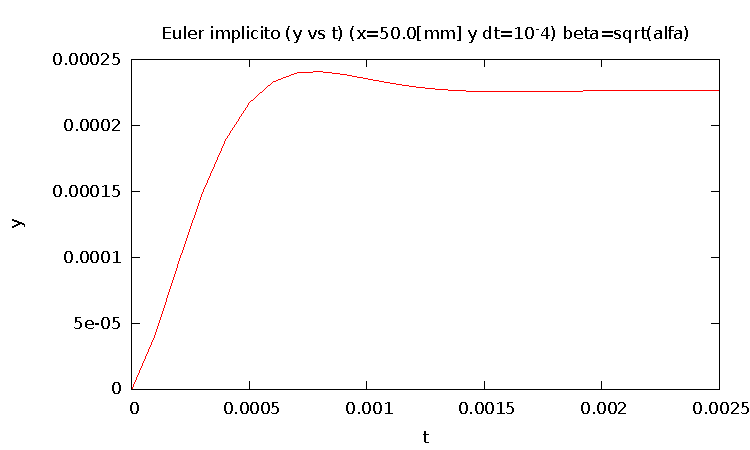
\includegraphics{./parte3/graficos/grafico_euler_S1_y_b1.pdf}
		\caption{Grafico de $y$ vs $t$ empleando un esquema de integración de Euler Implícito. $x=0.5[mm]$ y $\Delta t=10^{-4}$} 
		\label{fig:eulerS1b1_y}
	\end{subfigure}
	
	\begin{subfigure}[b]{0.8\textwidth}
		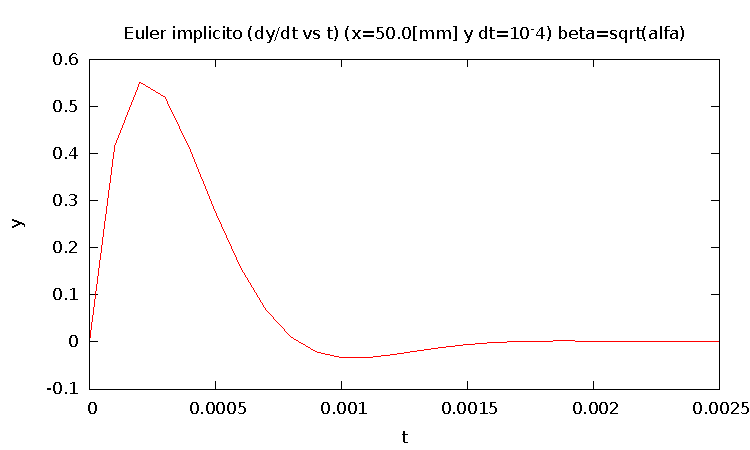
\includegraphics{./parte3/graficos/grafico_euler_S1_dy_b1.pdf}
		\caption{Grafico de $dy/dt$ vs $t$ empleando un esquema de integración de Euler Implícito. $x=0.5[mm]$ y $\Delta t=10^{-4}$} 
		\label{fig:eulerS1b1_dy}
	\end{subfigure}
\caption{Simulación 1: Solución numérica empleando Euler Implícito para $\beta=\sqrt{\alpha}$ } \label{euler_S1_b1}
\end{figure}
\end{center}

\begin{center}
\begin{figure} [H]
	\begin{subfigure}[b]{0.8\textwidth}
		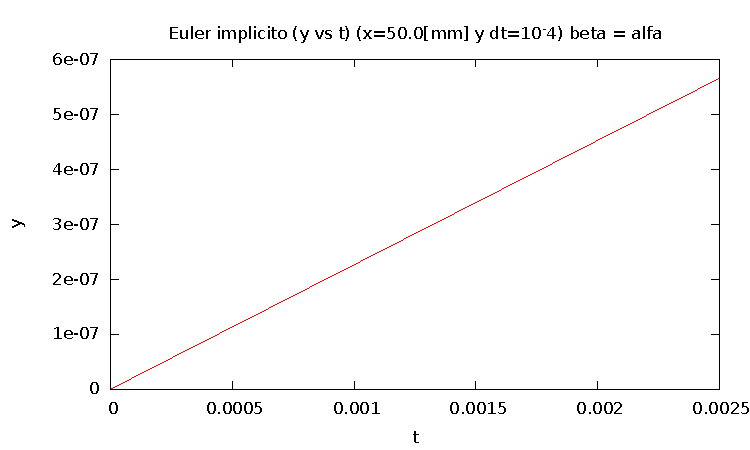
\includegraphics{./parte3/graficos/grafico_euler_S1_y_b2.pdf}
		\caption{Grafico de $y$ vs $t$ empleando un esquema de integración de Euler Implícito. $x=0.5[mm]$ y $\Delta t=10^{-4}$} 
		\label{fig:eulerS1b2_y}
	\end{subfigure}
	
	\begin{subfigure}[b]{0.8\textwidth}
		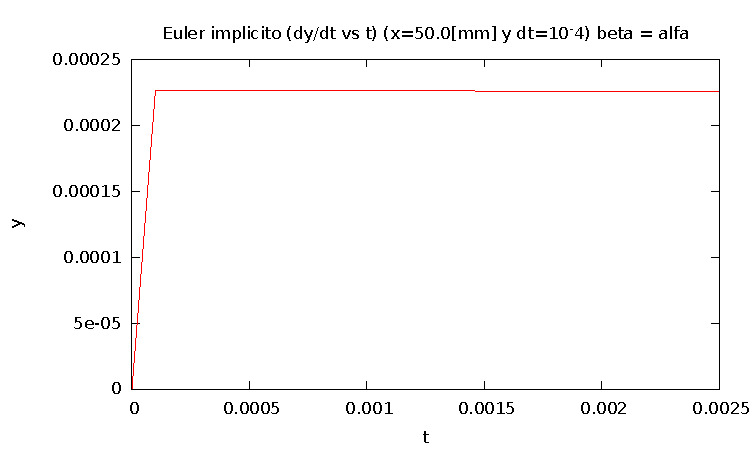
\includegraphics{./parte3/graficos/grafico_euler_S1_dy_b2.pdf}
		\caption{Grafico de $dy/dt$ vs $t$ empleando un esquema de integración de Euler Implícito. $x=0.5[mm]$ y $\Delta t=10^{-4}$} 
		\label{fig:eulerS1b2_dy}
	\end{subfigure}
\caption{Simulación 1: Solución numérica empleando Euler Implícito para $\beta=\alpha$ } \label{euler_S1_b2}
\end{figure}
\end{center}

%--------------------------------------------------------------------------

%----------------------- FIGURAS SIMULACION 1 -----------------------------
%----------------------- 	CRANK NICOLSON -----------------------------

\begin{center}
\begin{figure} [H]
	\begin{subfigure}[b]{0.8\textwidth}
		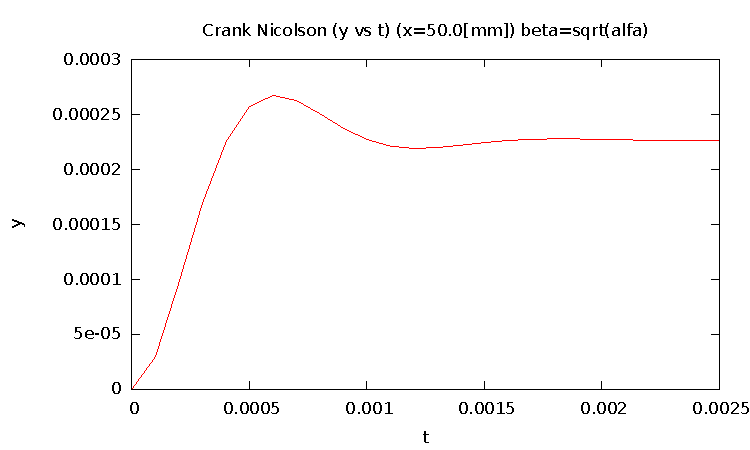
\includegraphics{./parte3/graficos/grafico_cn_S1_y_b1.pdf}
		\caption{Grafico de $y$ vs $t$ empleando un esquema de integración de Crank Nicolson. $x=0.5[mm]$ y $\Delta t=10^{-4}$} 
		\label{fig:cnS1b1_y}
	\end{subfigure}
	
	\begin{subfigure}[b]{0.8\textwidth}
		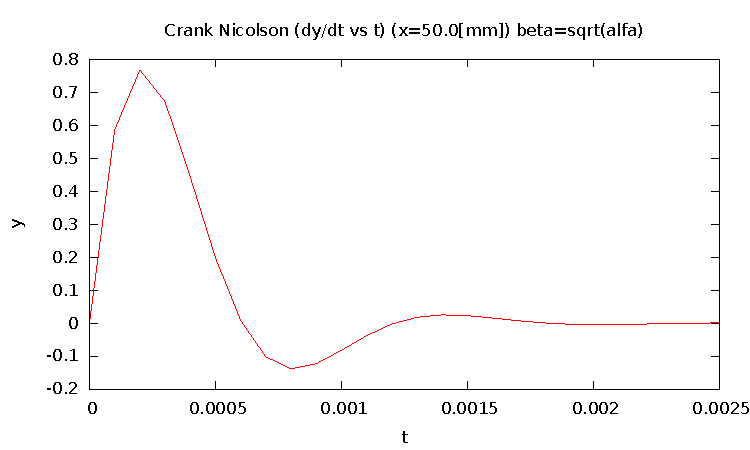
\includegraphics{./parte3/graficos/grafico_cn_S1_dy_b1.pdf}
		\caption{Grafico de $dy/dt$ vs $t$ empleando un esquema de integración de Crank Nicolson. $x=0.5[mm]$ y $\Delta t=10^{-4}$} 
		\label{fig:cnS1b1_dy}
	\end{subfigure}
\caption{Simulación 1: Solución numérica empleando Crank Nicolson para $\beta=\sqrt{\alpha}$ } \label{cn_S1_b1}
\end{figure}
\end{center}

\begin{center}
\begin{figure} [H]
	\begin{subfigure}[b]{0.8\textwidth}
		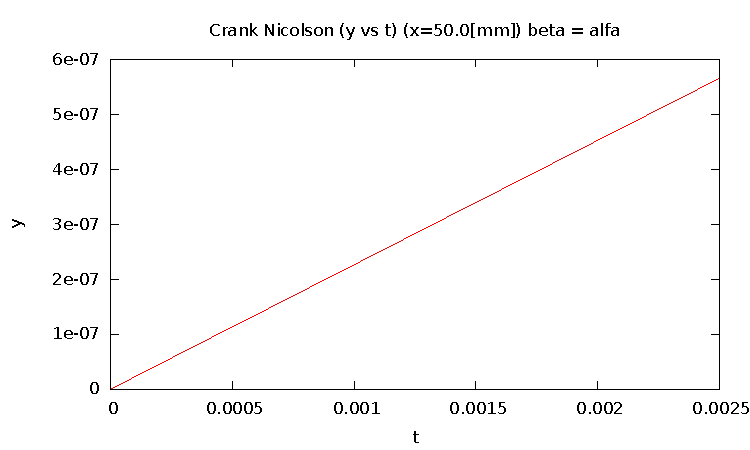
\includegraphics{./parte3/graficos/grafico_cn_S1_y_b2.pdf}
		\caption{Grafico de $y$ vs $t$ empleando un esquema de integración de Crank Nicolson. $x=0.5[mm]$ y $\Delta t=10^{-4}$} 
		\label{fig:cnS1b2_y}
	\end{subfigure}
	
	\begin{subfigure}[b]{0.8\textwidth}
		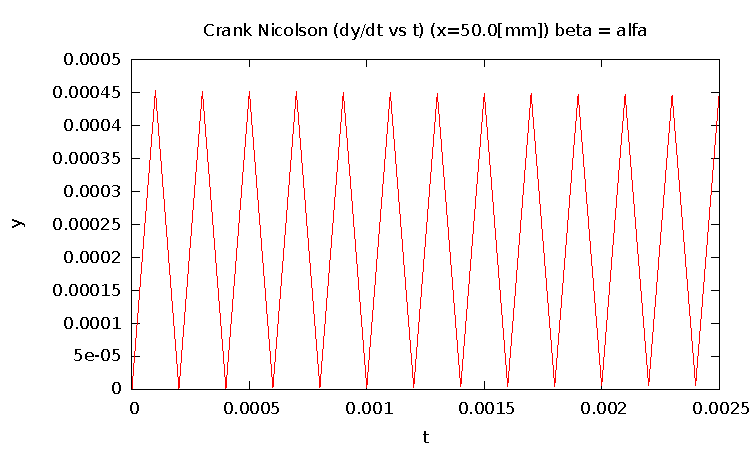
\includegraphics{./parte3/graficos/grafico_cn_S1_dy_b2.pdf}
		\caption{Grafico de $dy/dt$ vs $t$ empleando un esquema de integración de Crank Nicolson. $x=0.5[mm]$ y $\Delta t=10^{-4}$} 
		\label{fig:cnS1b2_dy}
	\end{subfigure}
\caption{Simulación 1: Solución numérica empleando Crank Nicolson para $\beta=\sqrt{\alpha}$ } \label{cn_S1_b2}
\end{figure}
\end{center}

%--------------------------------------------------------------------------

%----------------------- FIGURAS SIMULACION 2 -----------------------------
%----------------------- 	EULER IMPLICITO  -----------------------------

\begin{center}
\begin{figure} [H]
	\begin{subfigure}[b]{0.8\textwidth}
		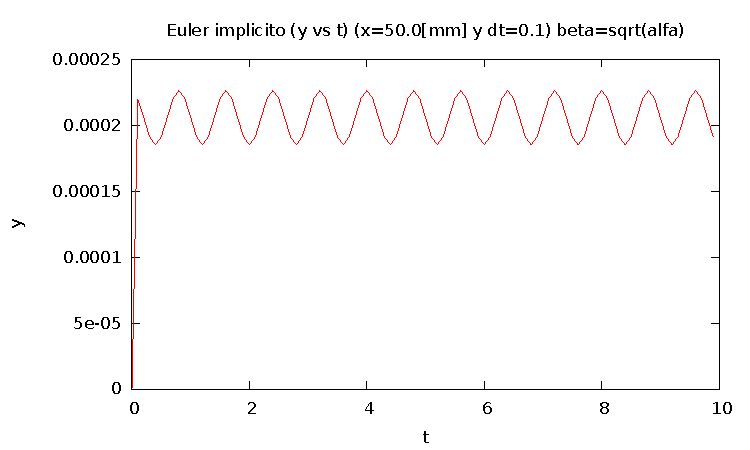
\includegraphics{./parte3/graficos/grafico_euler_S2_y_b1.pdf}
		\caption{Grafico de $y$ vs $t$ empleando un esquema de integración de Euler Implícito. $x=0.5[mm]$ y $\Delta t=0.1$} 
		\label{fig:eulerS2b1_y}
	\end{subfigure}
	
	\begin{subfigure}[b]{0.8\textwidth}
		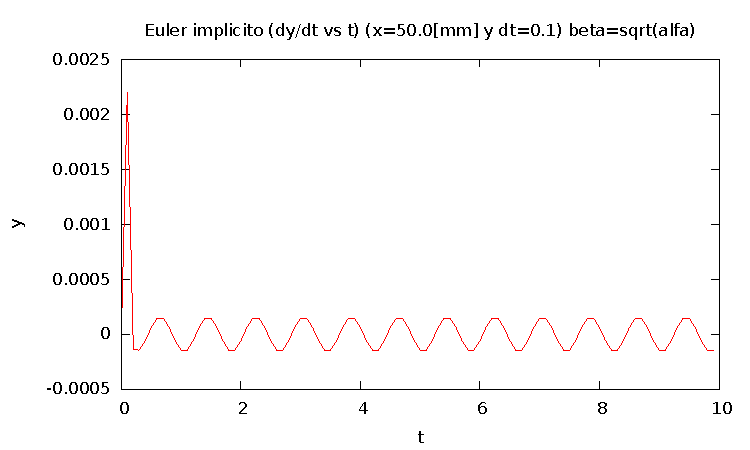
\includegraphics{./parte3/graficos/grafico_euler_S2_dy_b1.pdf}
		\caption{Grafico de $dy/dt$ vs $t$ empleando un esquema de integración de Euler Implícito. $x=0.5[mm]$ y $\Delta t=0.1$}  
		\label{fig:eulerS2b1_dy}
	\end{subfigure}
\caption{Simulación 2: Solución numérica empleando Euler Implícito para $\beta=\alpha$}
\end{figure}
\end{center}

\begin{center}
\begin{figure} [H]
	\begin{subfigure}[b]{0.8\textwidth}
		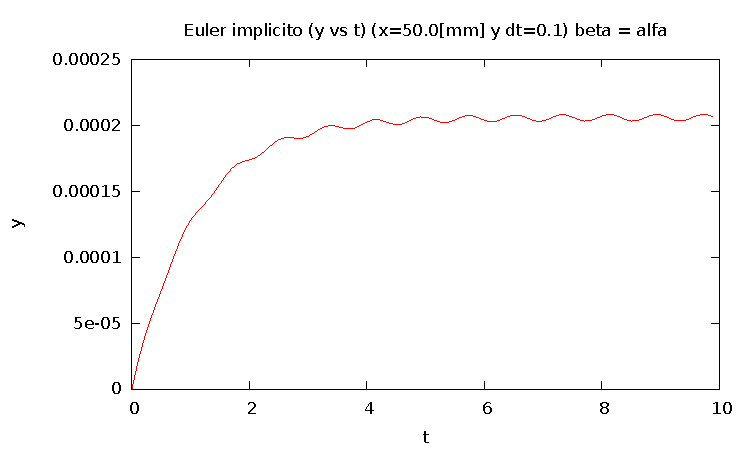
\includegraphics{./parte3/graficos/grafico_euler_S2_y_b2.pdf}
		\caption{Grafico de $y$ vs $t$ empleando un esquema de integración de Euler Implícito. $x=0.5[mm]$ y $\Delta t=0.1$} 
		\label{fig:eulerS2b2_y}
	\end{subfigure}
	
	\begin{subfigure}[b]{0.8\textwidth}
		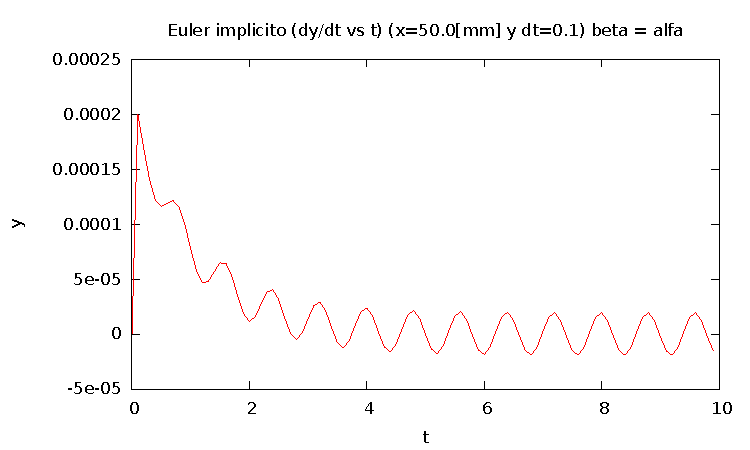
\includegraphics{./parte3/graficos/grafico_euler_S2_dy_b2.pdf}
		\caption{Grafico de $dy/dt$ vs $t$ empleando un esquema de integración de Euler Implícito. $x=0.5[mm]$ y $\Delta t=0.1$} 
		\label{fig:eulerS2b2_dy}
	\end{subfigure}
\caption{Simulación 2: Solución numérica empleando Euler Implícito para $\beta=\sqrt{\alpha}$}
\end{figure}
\end{center}

%--------------------------------------------------------------------------

%----------------------- FIGURAS SIMULACION 2 -----------------------------
%-----------------------	CRANK NICOLSON -----------------------------

\begin{center}
\begin{figure} [H]
	\begin{subfigure}[b]{0.8\textwidth}
		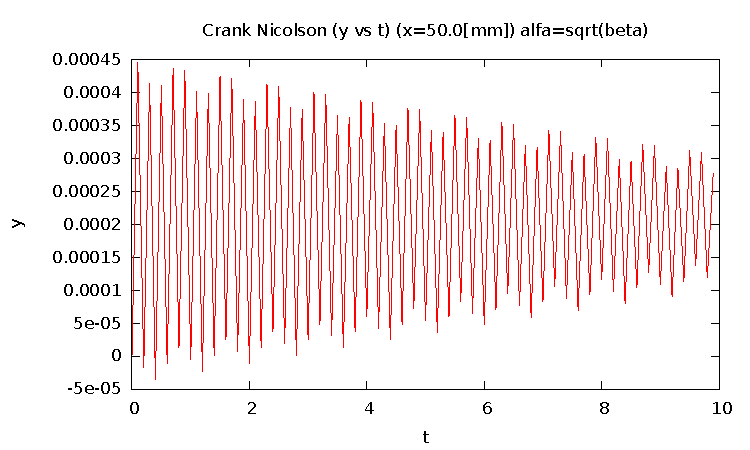
\includegraphics{./parte3/graficos/grafico_cn_S2_y_b1.pdf}
		\caption{Grafico de $y$ vs $t$ empleando un esquema de integración de Crank Nicolson. $x=0.5[mm]$ y $\Delta t=0.1$}  
		\label{fig:cnS2b1_y}
	\end{subfigure}
	
	\begin{subfigure}[b]{0.3\textwidth}
		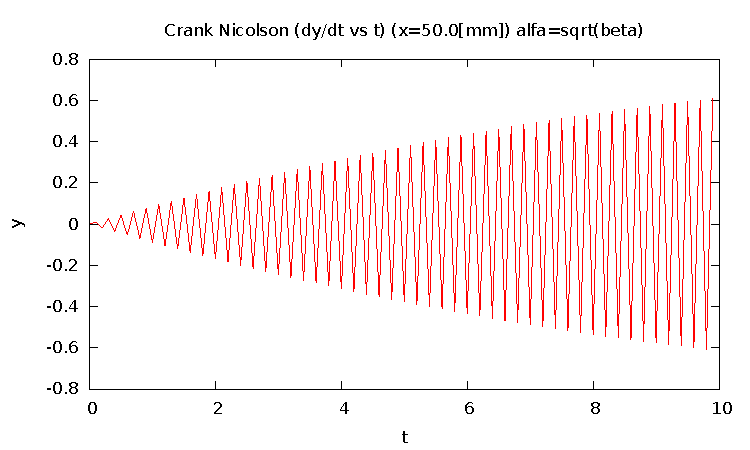
\includegraphics{./parte3/graficos/grafico_cn_S2_dy_b1.pdf}
		\caption{Grafico de $dy/dt$ vs $t$ empleando un esquema de integración de Crank Nicolson. $x=0.5[mm]$ y $\Delta t=0.1$}   
		\label{fig:cnS2b1_dy}
	\end{subfigure}
\caption{Simulación 2: Solución numérica empleando Crank Nicolson para $\beta=\alpha$}
\end{figure}
\end{center}

\begin{center}
\begin{figure} [H]
	\begin{subfigure}[b]{0.8\textwidth}
		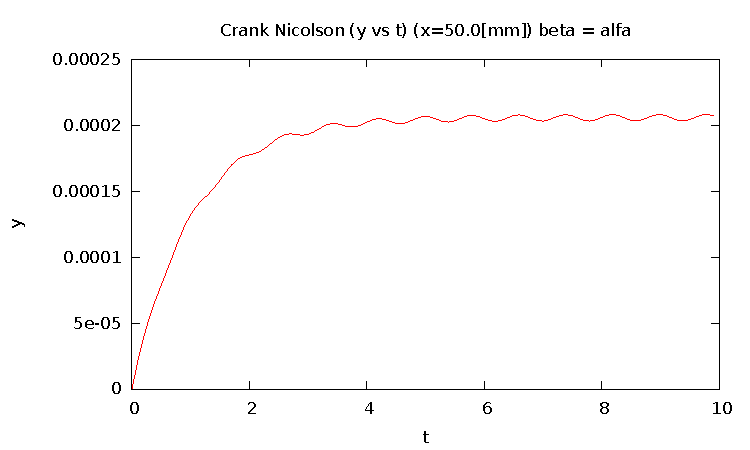
\includegraphics{./parte3/graficos/grafico_cn_S2_y_b2.pdf}
		\caption{Grafico de $y$ vs $t$ empleando un esquema de integración de Crank Nicolson. $x=0.5[mm]$ y $\Delta t=0.1$}  
		\label{fig:cnS2b2_y}
	\end{subfigure}
	
	\begin{subfigure}[b]{0.8\textwidth}
		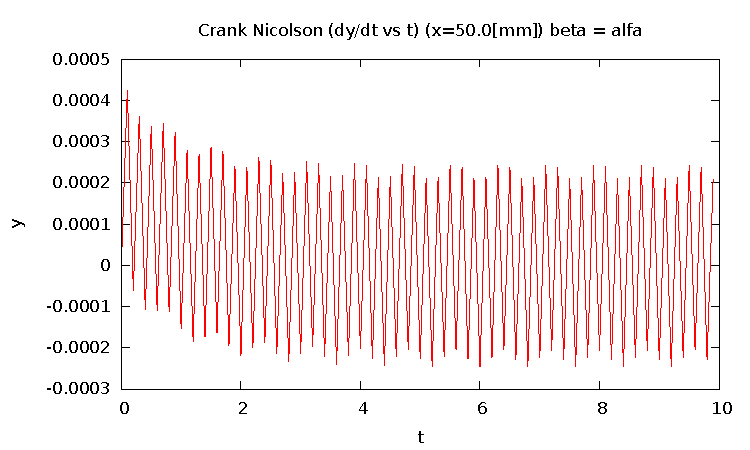
\includegraphics{./parte3/graficos/grafico_cn_S2_dy_b2.pdf}
		\caption{Grafico de $dy/dt$ vs $t$ empleando un esquema de integración de Crank Nicolson. $x=0.5[mm]$ y $\Delta t=0.1$} 
		\label{fig:cnS2b2_dy}
	\end{subfigure}
\caption{Simulación 2: Solución numérica empleando Crank Nicolson para $\beta=\sqrt{\alpha}$}
\end{figure}

\end{center}

%------------------------------------------------------------------------ 

\newpage
%Estudio del comportamiento mecánico de una arteria

\subsection{Parte 2: Un modelo hiperbólico para la interacción de la sangre con la pared}

Si para el mismo fenomeno descrito en la Parte 1 no se desprecia la interacción axial entre los anillos, entonces la ecuación (\ref{PROBLEMA_PARTE_2}) se modifica resultado en,

\begin{equation} \label{PROBLEMA_PARTE_2_2}
\dfrac{\partial^2 u}{\partial t^2} - \gamma^2 \dfrac{\partial^2 u}{\partial x^2} = f \hspace{0,5cm} x \in ] \alpha , \beta [
\end{equation}

Se denota la coordenada longitudinal $x$. $\sigma_x$ es la componente radial del esfuerzo axial y $L$ es el largo del cilindro considerado. Despreciando el factor de $y$ de la ecuación (\ref{PROBLEMA_PARTE_2_2}) y considerando $p-p_0 = f$ entonces se obtiene la ecuación de onda en una dimensión

\begin{equation} \label{E_ONDA}
\dfrac{\partial^2 u}{\partial t^2} - \gamma \dfrac{\partial^2 u}{\partial x^2} = f
\end{equation}

Se emplean los esquemas de Leap-Frog y Newmark para discretizar la ecuación anterior.

\subsubsection{Simulación 1: Leap-Frog}

El termino fuente utilizado para la simulación es $ f = ( 1 + \pi^2 \gamma^2 ) e^{-t} sin( \pi x ) $. Empleando un esquema de diferencias centradas en el espacio,

\begin{equation}
\dfrac{ \partial^2 u }{ \partial t^2 } = \gamma^2 \dfrac{ u_{j+1}^n - 2 u_j^n + u_{j-1}^n }{ \Delta x ^2} + 
 ( 1 + \pi^2 \gamma^2 ) e^{-t} sin( \pi x_j ) 
\end{equation}

Se utiliza un esquema de integración de Leap-Frog,

\begin{equation}
u^{n+1}_j - 2u^n_j + u^{n-1} = (\gamma \lambda)^2 ( u^n_{j-1} -2 u^n_j + u^n_{j+1} ) + f^n_j
\end{equation}

donde $\lambda=\dfrac{\Delta t}{\Delta x}$

Se estudia la estabilidad del método: 

\subsubsection*{Discretización espacial}

Se realiza una descomposición modal

\begin{align*}
S e ^ { i k_j p \Delta x } &= \dfrac{\gamma^2}{\Delta x^2} \left( e ^ { i k_j (p+1) \Delta x } - 2 e ^ { i k_j p \Delta x } + e ^ { i k_j (p-1) \Delta x } \right) \\
&= \underbrace{\dfrac{2 \gamma^2}{\Delta x^2} \left( cos(k_j \Delta x) - 1 \right)}_{\Omega_j} e ^ { i k_j p \Delta x}
\end{align*}

Es decir,

\begin{equation} \label{OMEGA_LF}
\Omega_j = \dfrac{2 \gamma^2}{\Delta x^2} \left( cos(k_j \Delta x) - 1 \right)
\end{equation}

Notar que $\Omega = \Re(\Omega_j)$. Se debe cumplir que

\begin{equation}
\Re(\Omega_j) \leq 0
\end{equation}

luego,

\begin{equation}
\Big| \dfrac{2 \gamma^2 }{ \Delta^2 } \leq 0
\end{equation}

\begin{equation}
\dfrac{-4 \gamma^2}{\Delta x^2} \leq \Re(\Omega_j) \leq 0
\end{equation}

\subsubsection*{Discretización temporal}

Estudia la estabilidad en el tiempo: se reemplaza $u_{j} = \omega$

\begin{equation}
\dfrac{\omega^{n+1} -2\omega^{n} + \omega^{n+1}}{\Delta t^2} = \vect{S} = \Omega_j \omega^n
\end{equation}

reeordenando

\begin{equation}
\omega^{n+1} - (\Omega_j \Delta t^2 +2) \omega^n + \omega^{n-1}
\end{equation}

utilizando $z_p$ (ver Sección ¿?, ecuación (¿?))

\begin{equation}
z_p^2 - \left( \Omega_j \Delta t^2 +2 \right) z_p + 1 = 0
\end{equation}

diviendo por $z_p$ (supuesto: $z_p \neq 0$, el estado transiente)

\begin{equation}
\left( \Omega_j \Delta t^2 + 2 \right) = \dfrac{1}{z_p} + z_p
\end{equation}

Se impone como solución $z_p = e^{i \theta}$ (notar que $|z_p| \leq 1$) . Reemplazando en la ecuación anterior,

\begin{equation}
\left( \Omega_j \Delta t^2 + 2 \right) = e^{i \theta} + e^{-i \theta} = 2 cos(\theta)
\end{equation}

La estabilidad se consigue acotando el lado izquierdo de la ecuación, obteniendo

\begin{equation}
-4 \leq \Re(\Omega_j \Delta t^2) \leq 0 
\end{equation}

reemplazando $\Omega_j$ obtenido de la ecuación (\ref{OMEGA_LF}) y considerando $\Omega_j = \Re (\Omega_j)$ resulta,

\begin{equation}
-4 \leq \dfrac{\gamma^2 \Delta t^2}{\Delta x^2} \left( cos(k_j \Delta x) - 1 \right)  \leq 0
\end{equation}

El criterio de estabilidad es

\begin{equation}
\dfrac{\gamma^2 \Delta t^2}{\Delta x^2} \leq 2
\end{equation}

$\gamma^2 \Delta t^2 / \Delta x^2 $ se puede interpretar como $(CFL)^2$ donde $CFL$ es el número de Courant-Friedrichs-Lewy

PENDIENTE -ESCRIBI LAS ECUACIONES, FALTA EXPLICARLAS !!!!!!!!!!!!!!!!

\subsubsection{Simulación 1: Newmark}

De la ecuacion (¿?) (Sección 1) se tiene $\partial u / \partial t = v$

\begin{equation}
\dfrac{\partial v}{\partial t} = \gamma ^2 \left[ \Theta \left( \dfrac{ u_{j+1}^{n+1} -2u_{j}^{n+1} + u_{j-1}^{n+1} }{\Delta x^2} \right) - (1-\Theta) \left( \dfrac{ u_{j+1}^{n} -2u_{j}^{n} + u_{j-1}^{n} }{\Delta x^2} \right) \right]
\end{equation} 

\subsubsection{Discretización espacial}

Se utiliza $\Theta=0.5$ (Esquema Crank Nicolson)

\begin{equation}
\dfrac{\partial v}{\partial t} = \left[ \left( \vect{S} e^{i k_j p \Delta x} \right)^{n+1} + \left( \vect{S} e^{i k_j p \Delta x} \right)^{n}  \right]
\end{equation}

Se resulve $(\vect(S))^n$

\begin{align*}
S e ^ { i k_j p \Delta x } &= \dfrac{\gamma^2}{2 \Delta x^2} \left( e ^ { i k_j (p+1) \Delta x } - 2 e ^ { i k_j p \Delta x } + e ^ { i k_j (p-1) \Delta x } \right) \\
&= \underbrace{\dfrac{\gamma^2}{\Delta x^2} \left( cos(k_j \Delta x) - 1 \right)}_{\Omega_j} e ^ { i k_j p \Delta x}
\end{align*}

es decir,

\begin{equation} \label{OMEGA_j}
\Omega_j = \dfrac{\gamma^2}{\Delta x^2} \left( cos(k_j \Delta x) - 1 \right)
\end{equation}

\begin{equation} \label{CONDICION_OMEGA_j_NM}
\dfrac{-2 \gamma^2}{\Delta x^2} \leq \Re(\Omega_j) \leq 0
\end{equation}

Se obtiene el mismo resultado para $(\vect(S))^{n+1}$, Sumando $(\vect(S))^{n+1} + (\vect(S))^{n}$ luego obtenemos la mismas ecuación obtenida en la discretización Leap-Frog. Por lo tanto, la condición de $\Re(\Omega_j')$ ($\Omega_j' = \Omega_j^{n+1} + \Omega_j^{n}$)

\begin{equation}
\dfrac{-4 \gamma^2}{\Delta x^2} \leq \Re(\Omega_j') \leq 0
\end{equation}

Como $u_j$ y $v_j$ emplean diferencias finitas centradas se obtienen los mismos valores propios de $\vect{S}$

\subsubsection*{Discretización temporal}

Se integra la ecuación $\partial v / \partial t$. Se utiliza la notación $v_j = \omega$

\begin{equation}
\dfrac{\omega^{n+1}-\omega^n}{\Delta t} = \Omega_j^{n+1} \omega^{n+1} + \Omega_j^{n} \omega^{n}
\end{equation}

agrupando términos

\begin{equation}
\omega^{n+1} = \underbrace{ \dfrac{1+\Omega_j \Delta t}{1-\Omega_j \Delta t} }_{z_p} \omega^n
\end{equation}

como $\Omega_j = \Re(\Omega_j)$, entonces

\begin{equation} \label{zp_nm_v}
z_p = \dfrac{ 1 + \Omega_j }{ 1-\Omega_j}
\end{equation}

tomando en cuenta la condición \ref{CONDICION_OMEGA_j_NM} se verifica que

\begin{equation}
-1 \leq z_p \leq 1
\end{equation}




%----

\subsection{Atractor de Lorenz}
%ATRACTOR DE LORENZ
El sistema de ecuaciones de Lorenz es un ejemplo de un sistema de ecuaciones diferenciales de orden 1, tridimensional, no lineal, que tiene un comportamiento caótico para algunos valores de sus parámetros. Este sistema de ecuaciones permite modelar los rollos de convección que se producen en la atmosfera terrestre. Es un modelo simplificado de la convección de Rayleigh-Benard (ecuaciones de Navier-Stokes con hipótesis de Boussinesq).
\begin{equation}
\left\{ 
\begin{matrix}
dx/dt =& Pr (y(t) - x(yt)) \\
dy/dt =& Ra x(t) - y(t) - x(t)z(t) \\
dz/dt =& x(t) y(t) - \beta z(t)
\end{matrix} \right.
\end{equation}
Donde $Pr$ es el número de Prandtl y $Ra$ es el número de Rayleigh. Las variables dinámicas $x$, $y$ y $z$ represetan el estado del sistema a cada instante $t$:

\begin{itemize}
\item x(t) es proporcional a la intensidad del movimiento de convección  
\item y(t) es proporcional a la diferencia de temperatura entre las corrientes ascendentes y descendentes
\item z(t) es proporcional a la diferencia entre el perfil vertical de temperatura y un perfil vertical de temperatura lineal
\end{itemize}

Los sistemas dinámicos son sistemas que son función del tiempo. Que sea caótico significa que varia de manera no lineal y a su vez que el sistema presenta sensibilidad a frente a los parámetros entrada. Además presentan un comportamiento oscilante, pudiendo ser periodico o no periodico. \\

\subsubsection{Parte 1}
Las Figuras \ref{lorenz1} y \ref{lorenz2} reproducen los gráficos del articulo \textit{Deterministic Nonperiodic Flow} de Lorenz
\begin{figure} [H]
\begin{center}
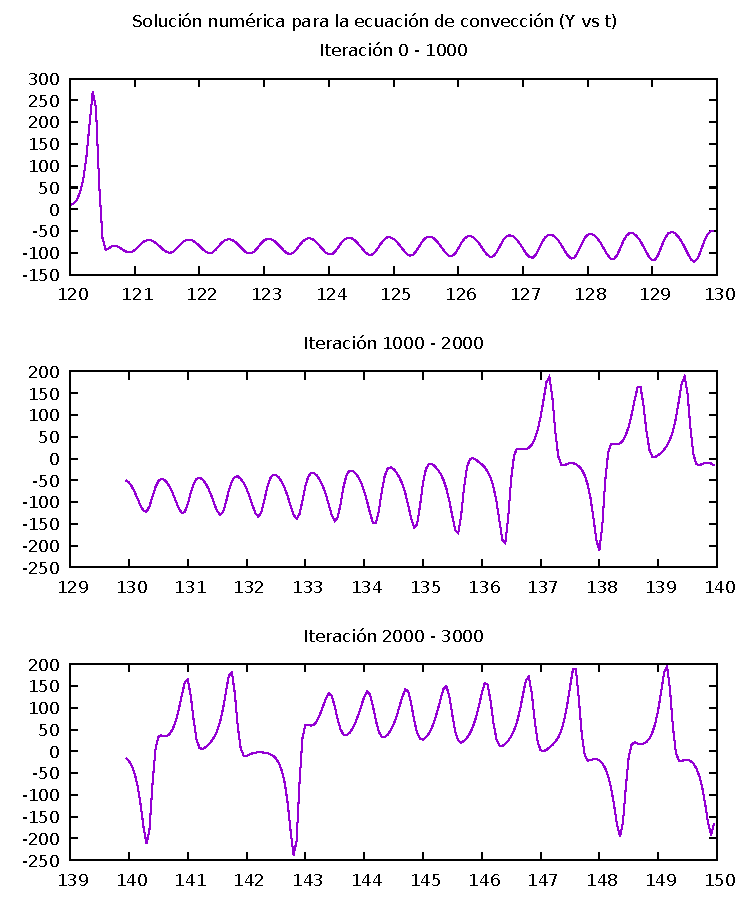
\includegraphics[width=0.8\textwidth]{./parte4/graficos/FIGURA1.pdf}
\caption{} \label{lorenz1}
\end{center}
\end{figure}

\begin{figure} [H]
\begin{center}
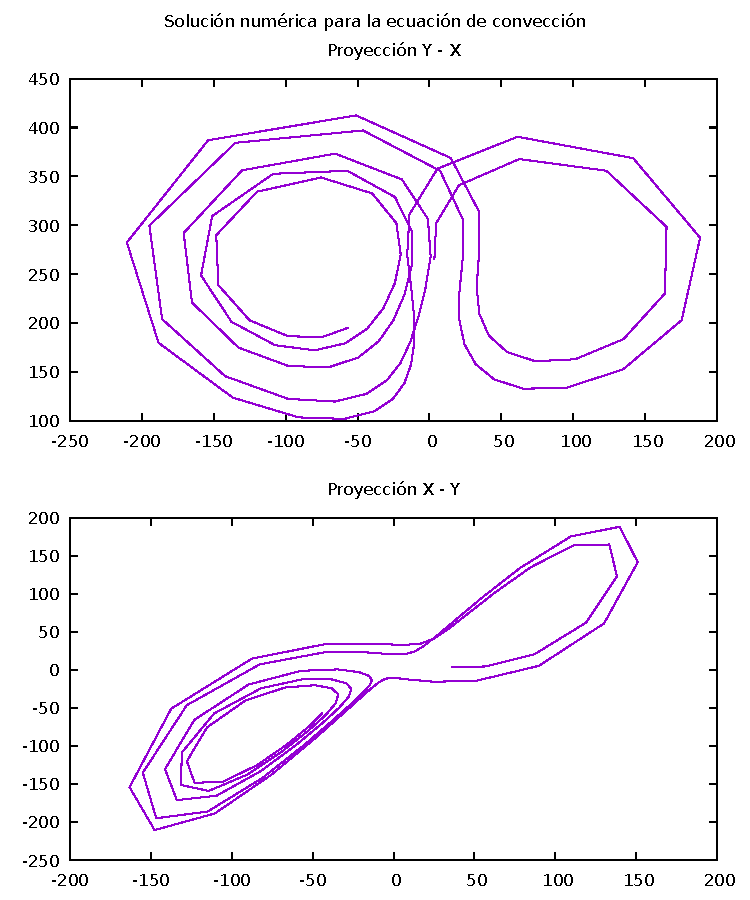
\includegraphics[width=0.8\textwidth]{./parte4/graficos/FIGURA2.pdf}
\caption{} \label{lorenz2}
\end{center}
\end{figure}

%---------------------------

\subsubsection{Parte 2}

Se grafica la solución a la ecuación de convección utilizando los siguientes valores: $Pr=10$, $\beta= 8/3$ y $Ra = 0.5 \, , \, 10 , \, 28$ 

\begin{figure} [H]
\begin{center}
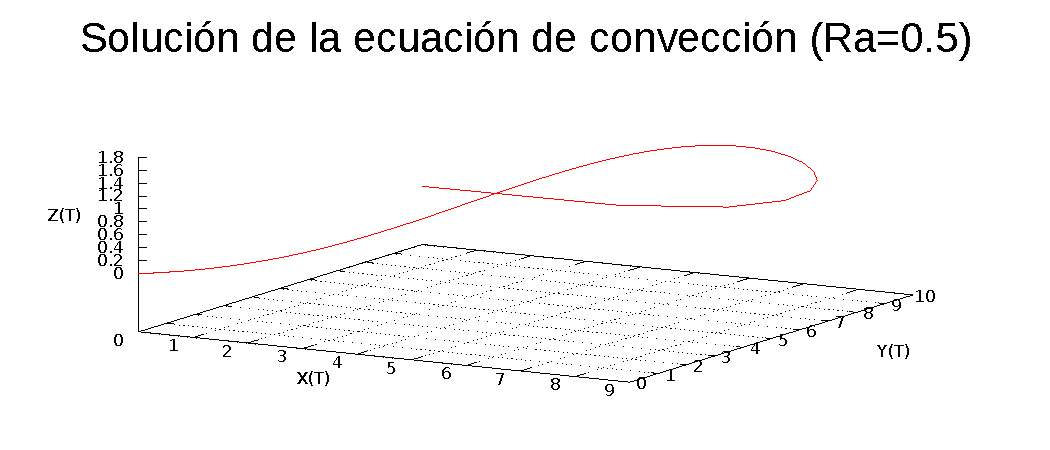
\includegraphics[width=0.8\textwidth]{./parte4/graficos/grafico_P3_3d_ra05.pdf}
\caption{}
\end{center}
\end{figure}

\begin{figure} [H]
\begin{center}
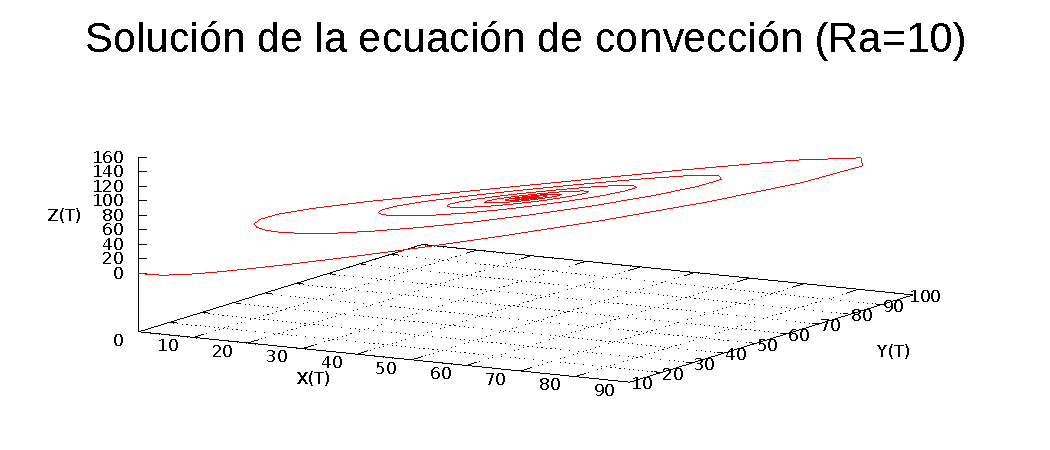
\includegraphics[width=0.8\textwidth]{./parte4/graficos/grafico_P3_3d_ra10.pdf}
\caption{}
\end{center}
\end{figure}

\begin{figure} [H]
\begin{center}
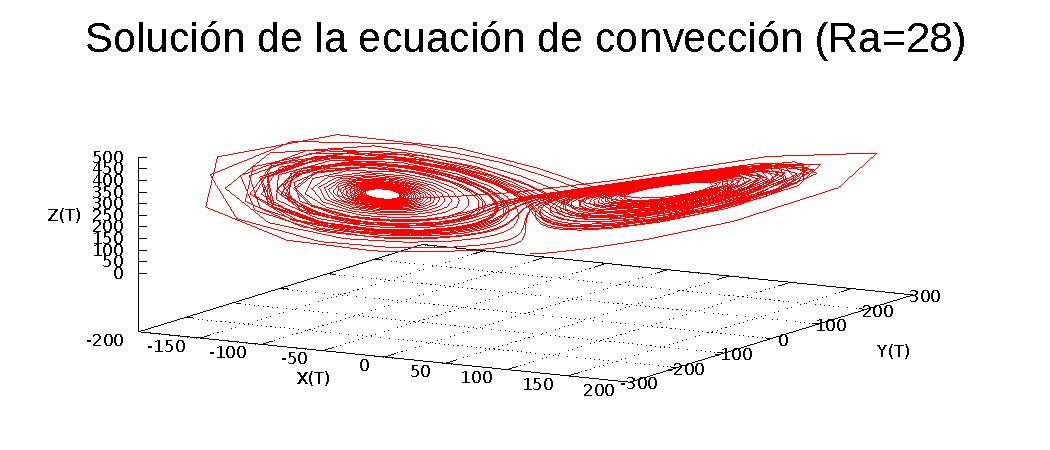
\includegraphics[width=0.8\textwidth]{./parte4/graficos/grafico_P3_3d_ra28.pdf}
\caption{}
\end{center}
\end{figure}

%---------------------------

\subsubsection{Parte 3}
Haciendo variar paulatinamente $Ra$ entre 0 y 30

\begin{figure} [H]
\hspace{-1cm} 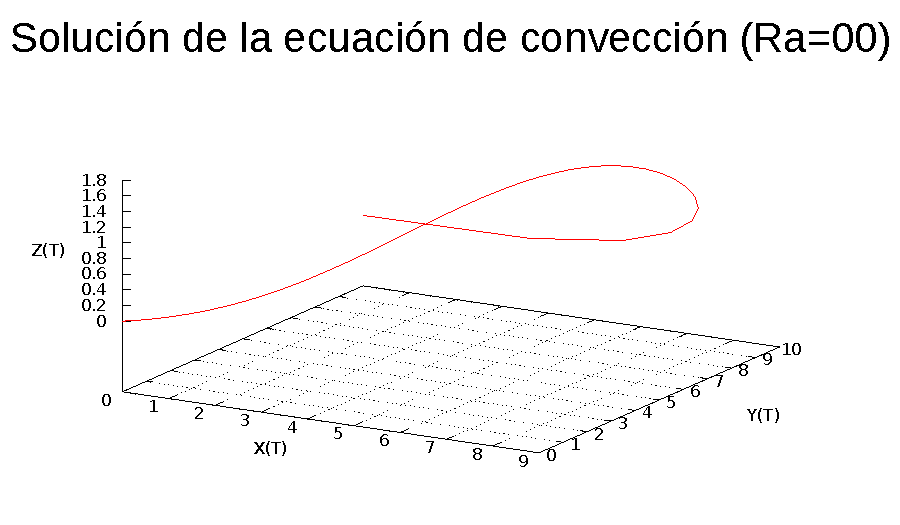
\includegraphics[width=0.6\textwidth]{./parte4/graficos/grafico_P3_3d_ra00.pdf}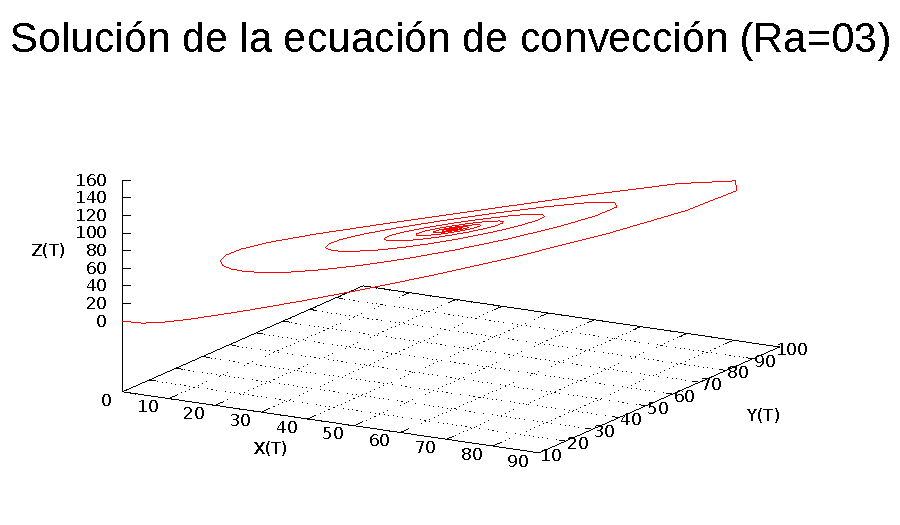
\includegraphics[width=0.6\textwidth]{./parte4/graficos/grafico_P3_3d_ra03.pdf}
\caption{} 
\end{figure}

\begin{figure} [H]
\hspace{-1cm} 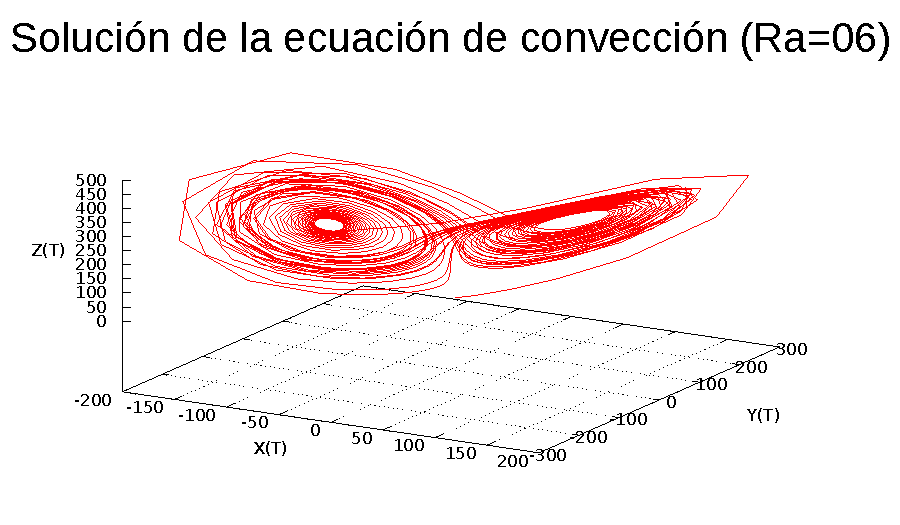
\includegraphics[width=0.6\textwidth]{./parte4/graficos/grafico_P3_3d_ra06.pdf}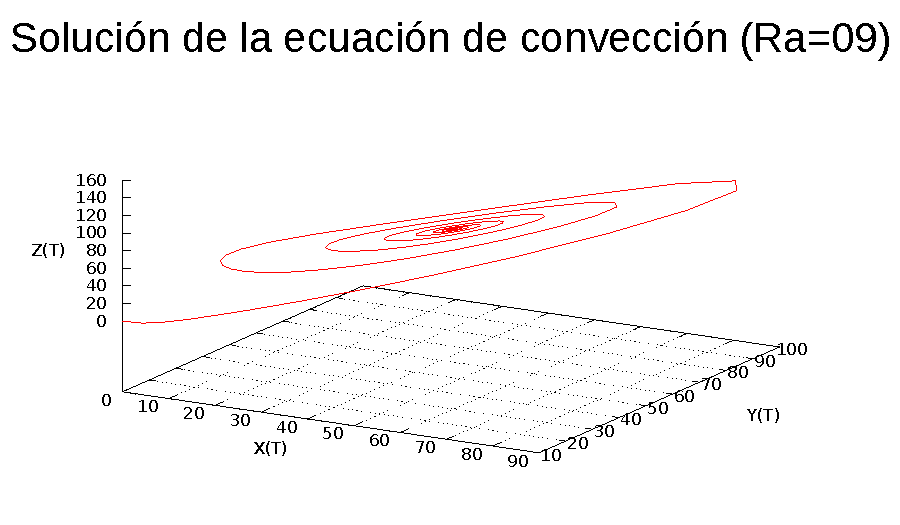
\includegraphics[width=0.6\textwidth]{./parte4/graficos/grafico_P3_3d_ra09.pdf}
\caption{} 
\end{figure}

\begin{figure} [H]
\hspace{-1cm} 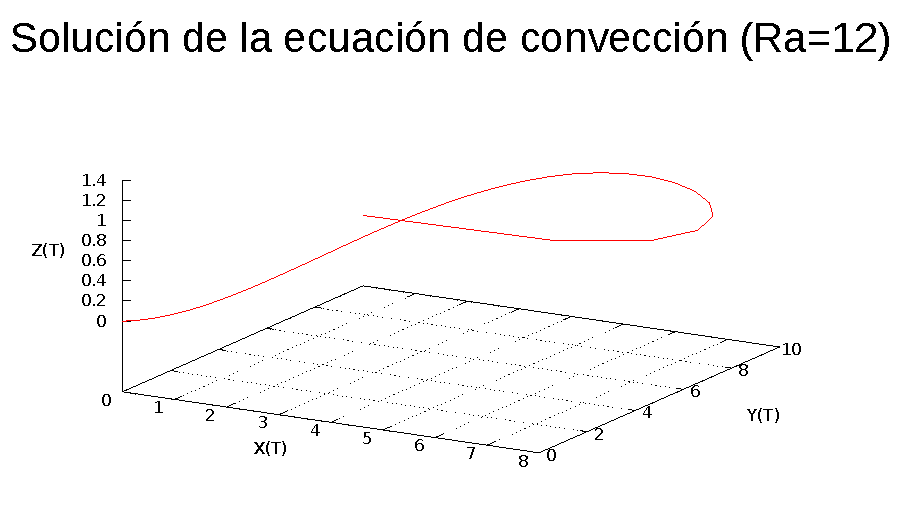
\includegraphics[width=0.6\textwidth]{./parte4/graficos/grafico_P3_3d_ra12.pdf}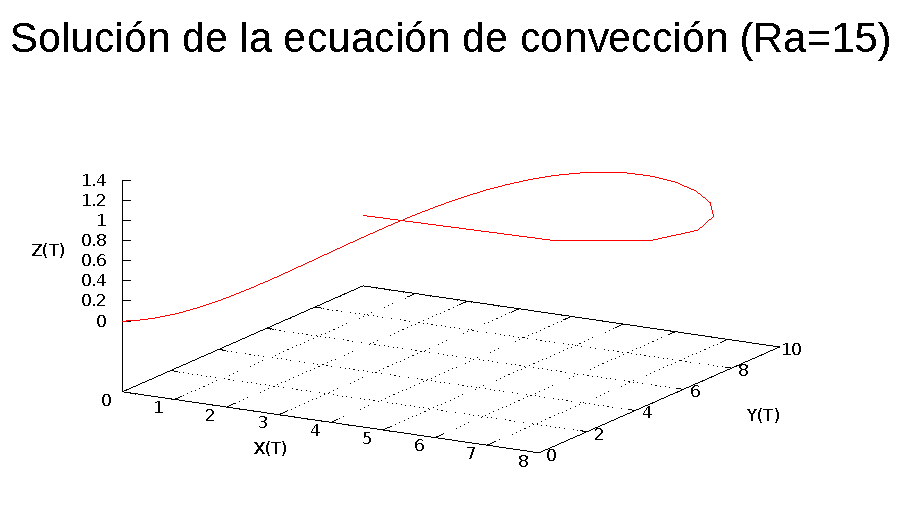
\includegraphics[width=0.6\textwidth]{./parte4/graficos/grafico_P3_3d_ra15.pdf}
\caption{} 
\end{figure}

\begin{figure} [H]
\hspace{-1cm} 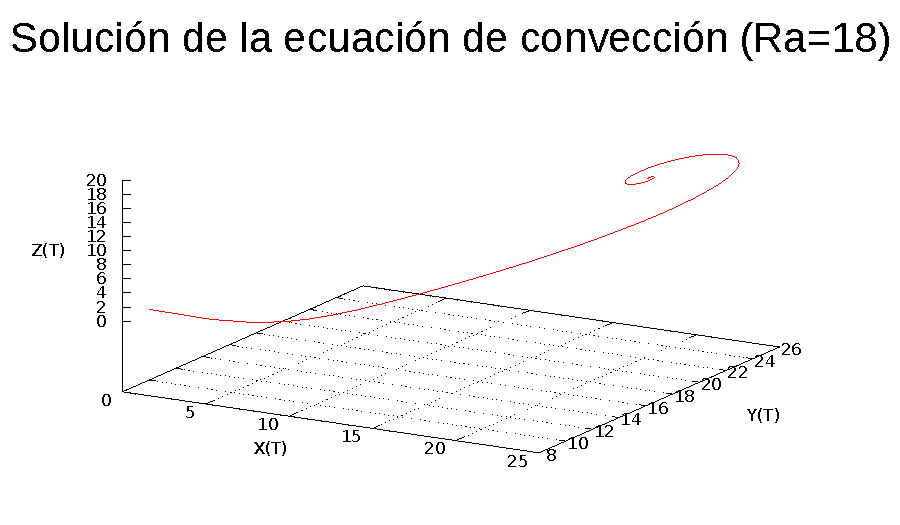
\includegraphics[width=0.6\textwidth]{./parte4/graficos/grafico_P3_3d_ra18.pdf}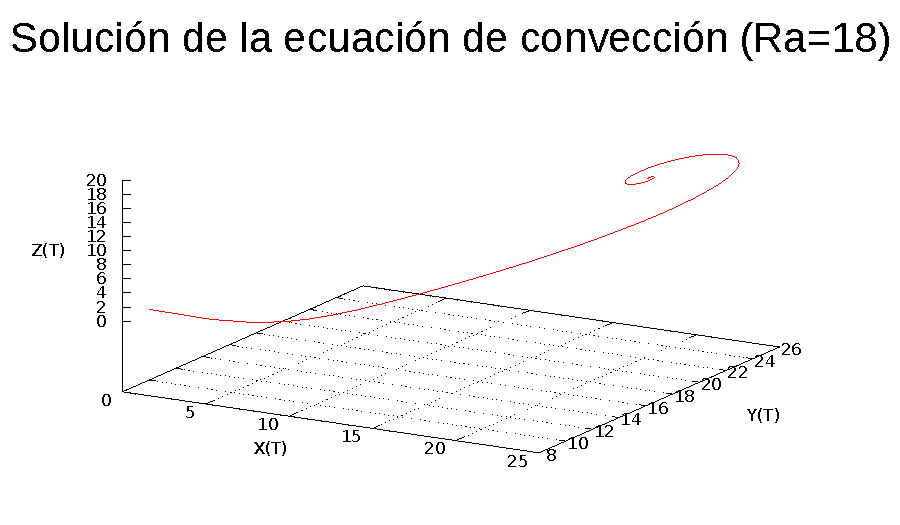
\includegraphics[width=0.6\textwidth]{./parte4/graficos/grafico_P3_3d_ra18.pdf}
\caption{} 
\end{figure}

\begin{figure} [H]
\hspace{-1cm} 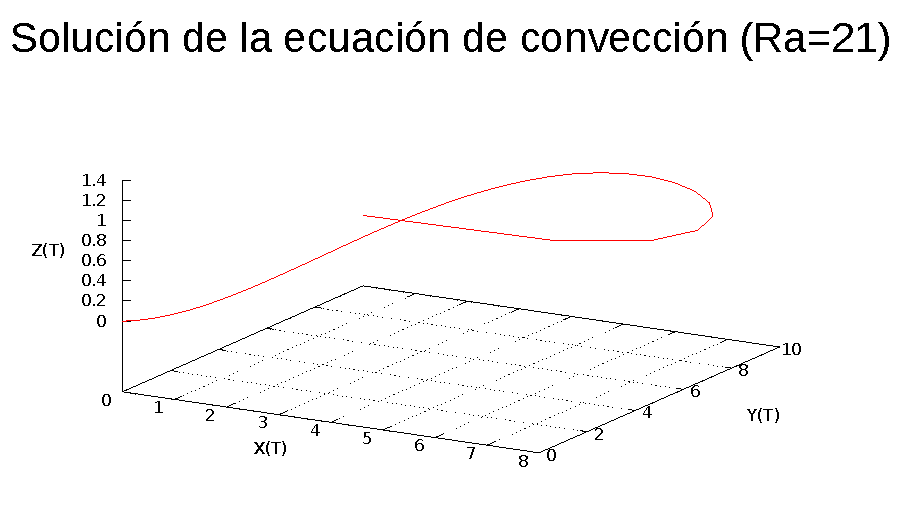
\includegraphics[width=0.6\textwidth]{./parte4/graficos/grafico_P3_3d_ra21.pdf}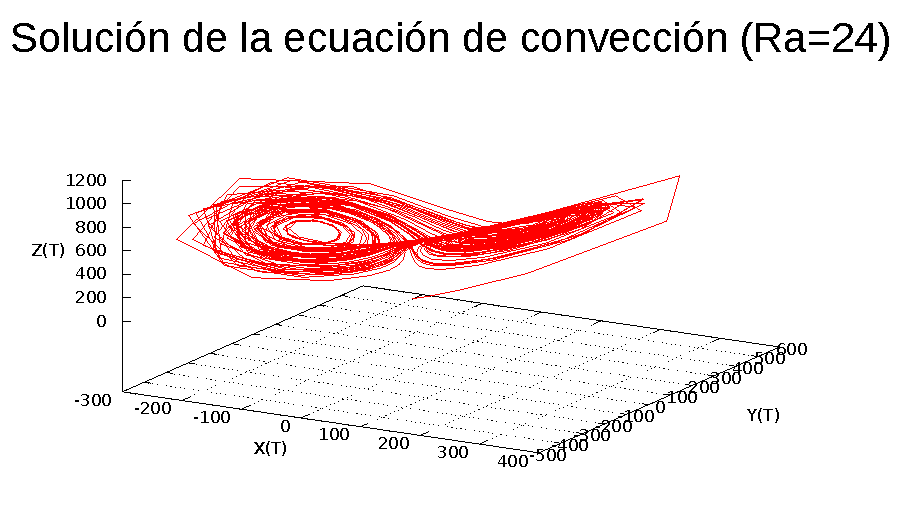
\includegraphics[width=0.6\textwidth]{./parte4/graficos/grafico_P3_3d_ra24.pdf}
\caption{} 
\end{figure}

\begin{figure} [H]
\hspace{-1cm} 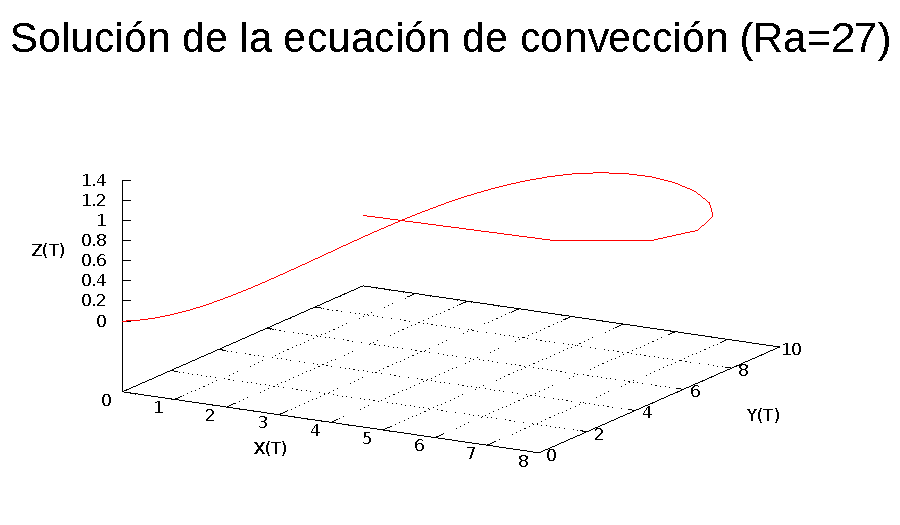
\includegraphics[width=0.6\textwidth]{./parte4/graficos/grafico_P3_3d_ra27.pdf}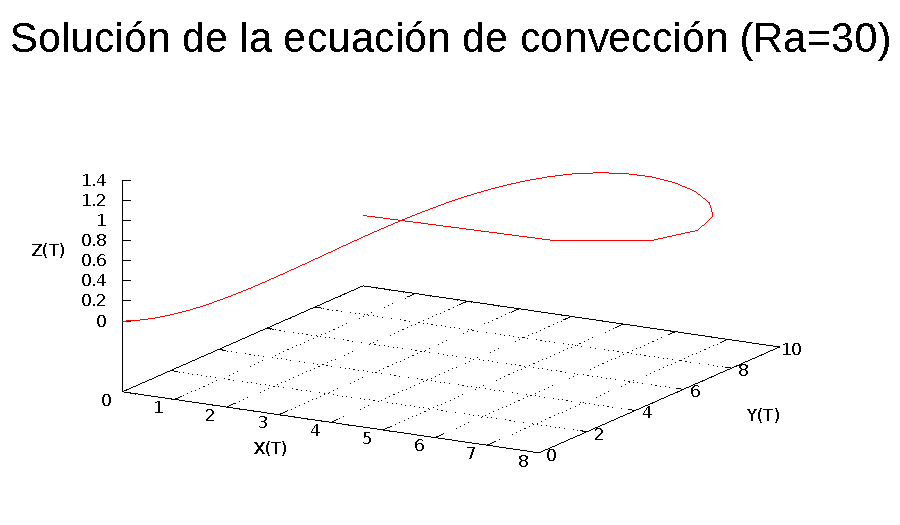
\includegraphics[width=0.6\textwidth]{./parte4/graficos/grafico_P3_3d_ra30.pdf}
\caption{} 
\end{figure}

\newpage
%---------------------------------------------

\section{Conclusiones y Observaciones}

\newpage
%---------------------------------------------

\begin{thebibliography}{3}

\bibitem{lorenz} \textsc{Lorenz, E.} , \textit{Deterministic Nonperiodic Flow}, Journal of the Atmospheric Science, vol. 20, pag. 130-141, 1963

\bibitem{fortran} \textsc{Chapman, S.} , \textit{Fortran 90/95 for Scientits and Engineers}, Ediforial Mcgraw-Hill, 2003, ISBN-13: 978-0072922387

\bibitem{num_mat} \textsc{Quarteroni, A.} , \textsc{Sacco, R.} y \textsc{Saleri, F.} , \textit{Numerical Mathematics},
Editorial Springer, 2000, ISBN 0-387-98959-5

\bibitem{met_num} \textsc{Chapra, S.} y \textsc{Canale, R.} , \textit{Métodos numéricos para ingenieros}, 5ta edición,
Editorial McGraw-Hill, 2007, ISBN-13: 978-970-10-6114-5
\end{thebibliography}

\end{document}
